% Motivation figure: how an agentic reviewer (e.g. Codex /review, Claude Code) reviews a PR,
% and why it is token-hungry: it calls the LLM once per tool turn, and every call re-sends the
% prompt plus every earlier tool result. Block sizes are schematic, not measurements.
% Build: latexmk -pdf motivation.tex
\documentclass[tikz,border=3pt]{standalone}
\usepackage[T1]{fontenc}
\usepackage[default]{sourcesanspro}
\usepackage[scaled=0.86]{beramono}
\usepackage{amsmath,amssymb}
\usepackage{fontawesome5}
\usetikzlibrary{calc,arrows.meta,positioning,decorations.pathreplacing,bending}

\definecolor{ink}{HTML}{111111}
\definecolor{grey}{HTML}{6B6B6B}
\definecolor{hair}{HTML}{BDBDBD}
\definecolor{badS}{HTML}{B03A2E}  \definecolor{badF}{HTML}{FBEDEB}
\definecolor{llmS}{HTML}{3D5A98}  \definecolor{llmF}{HTML}{EAEEF8}
\definecolor{outS}{HTML}{C55A11}  \definecolor{outF}{HTML}{FCEADF}
% prompt and tool results (each result keeps its colour in every later call)
\definecolor{cP}{HTML}{7FA0CF}
\definecolor{c1}{HTML}{F2A65A} \definecolor{c2}{HTML}{F6CF65} \definecolor{c3}{HTML}{9BCB7D}
\definecolor{c4}{HTML}{6CC0B5} \definecolor{c5}{HTML}{B49BD6} \definecolor{c6}{HTML}{E59AB8}

\tikzset{
  >={Triangle[length=2.4mm,width=2mm]},
  col/.style={draw=ink, line width=1.1pt, rounded corners=6pt},
  ttl/.style={font=\large\bfseries, text=ink, anchor=north west, inner sep=0pt},
  card/.style={draw=hair, fill=white, line width=0.7pt, rounded corners=4pt, align=center,
               font=\small\bfseries, text=ink, minimum width=2.7cm, minimum height=0.95cm},
  big/.style={->, line width=1.5pt, draw=ink},
}

\begin{document}
\begin{tikzpicture}

% ======================================================================== top row
% Input
\draw[col, fill=white] (0,0) rectangle (3.5,-4.4);
\node[ttl] at (0.25,-0.25) {Input};
\node[card] (prompt) at (1.75,-1.75) {{\color{cP}\faFile*}\; Prompt\\[-2pt]{\scriptsize\mdseries\color{grey}rubric, PR text, diff}};
\node[card] (repo)   at (1.75,-3.2) {{\color{grey}\faFolderOpen}\; Project folder\\[-2pt]{\scriptsize\mdseries\color{grey}the whole repository}};

% Agentic loop
\draw[col, draw=badS, fill=badF] (4.2,0) rectangle (13.3,-4.4);
\node[ttl] at (4.45,-0.25) {Agentic review \textmd{\normalsize\color{grey}(e.g., Codex \texttt{/review}, Claude Code)}};
\node[draw=llmS, fill=llmF, line width=1pt, rounded corners=5pt, minimum width=2.5cm, minimum height=1.3cm,
      align=center, font=\small\bfseries] (agent) at (6.0,-2.45) {{\Large\color{llmS}\faRobot}\\LLM agent};
\node[draw=ink, fill=white, line width=1pt, rounded corners=5pt, minimum width=2.5cm, minimum height=1.3cm,
      align=center, font=\small\bfseries] (tools) at (11.5,-2.45) {{\Large\color{grey}\faFolderOpen}\\Project folder};
\draw[->, line width=1.3pt, draw=ink] ([yshift=4pt]agent.north east) to[out=18, in=162]
  node[above, font=\scriptsize, align=center]{\textbf{tool call}\\[-2pt]{\ttfamily read\_file, grep, run tests}} ([yshift=4pt]tools.north west);
\draw[->, line width=1.3pt, draw=grey, dash pattern=on 4pt off 2.5pt] ([yshift=-4pt]tools.south west) to[out=198, in=-18]
  node[below, font=\scriptsize, align=center, text=grey]{\textbf{tool result}\\[-2pt]file contents, matches, logs} ([yshift=-4pt]agent.south east);
\node[circle, fill=badS, text=white, font=\small\bfseries, minimum size=0.95cm, align=center, inner sep=0pt]
  (rep) at (8.75,-2.45) {$\times n$};
\node[font=\scriptsize\bfseries, text=badS] at (8.75,-3.12) {turns};

% Output
\draw[col, draw=outS, fill=outF] (14.0,0) rectangle (17.5,-4.4);
\node[ttl] at (14.25,-0.25) {Output};
\node[card, minimum height=1.6cm] (out) at (15.75,-2.45) {{\Large\color{outS}\faClipboardList}\\Review findings};

\draw[big] (3.5,-1.75) -- ++(0.35,0) |- (agent.west |- 0,-2.2);
\draw[big] (3.5,-3.2) -- ++(0.35,0) |- (agent.west |- 0,-2.7);
\draw[big] (13.3,-2.45) -- (14.0,-2.45);

% ======================================================================== bottom: the token problem
\draw[col, draw=badS, fill=white] (0,-5.0) rectangle (17.5,-11.6);
\node[ttl] at (0.25,-5.25) {Problem: every turn is a new LLM call that re-sends everything before it};

% axes
\def\bx{1.3}\def\by{-10.85}\def\bw{0.72}\def\gap{0.38}\def\bh{0.4}
\draw[->, line width=0.8pt, draw=grey] (\bx-0.3,\by) -- (\bx-0.3,-6.45) node[above, anchor=south west, xshift=-4pt, font=\scriptsize, text=grey]{input tokens per call};
\draw[line width=0.8pt, draw=grey] (\bx-0.3,\by) -- (10.55,\by);

% columns: call k sends the prompt + results 1..k-1
\foreach \k in {1,...,7}{
  \pgfmathsetmacro{\x}{\bx+(\k-1)*(\bw+\gap)}
  \fill[cP] (\x,\by) rectangle ++(\bw,\bh);
  \pgfmathtruncatemacro{\m}{\k-1}
  \ifnum\m>0
    \foreach \j in {1,...,\m}{
      \pgfmathtruncatemacro{\cj}{mod(\j-1,6)+1}
      \fill[c\cj] (\x,\by+\j*\bh) rectangle ++(\bw,\bh);
      \draw[white, line width=0.6pt] (\x,\by+\j*\bh) -- ++(\bw,0);
    }
  \fi
  \node[font=\scriptsize, text=grey, below] at (\x+\bw/2,\by) {call \k};
}
\pgfmathsetmacro{\xd}{\bx+7*(\bw+\gap)}
\node[font=\large, text=grey] at (\xd+0.15,-9.6) {$\cdots$};
\pgfmathsetmacro{\xn}{\xd+0.6}
\fill[cP] (\xn,\by) rectangle ++(\bw,\bh);
\foreach \j in {1,...,9}{
  \pgfmathtruncatemacro{\cj}{mod(\j-1,6)+1}
  \fill[c\cj] (\xn,\by+\j*\bh) rectangle ++(\bw,\bh);
  \draw[white, line width=0.6pt] (\xn,\by+\j*\bh) -- ++(\bw,0);
}
\node[font=\scriptsize, text=grey, below] at (\xn+\bw/2,\by) {call $n$};

% annotations on the chart
\pgfmathsetmacro{\xa}{\bx+1*(\bw+\gap)}
\draw[<-, line width=0.9pt, draw=ink] (\xa+\bw/2,\by+2*\bh+0.05) -- ++(0,1.9)
  node[above, font=\scriptsize, align=center, inner sep=2pt]{the result of turn 1 (outlined)\\is sent again in every later call};
% outline the turn-1 result wherever it is re-sent
\foreach \k in {2,...,7}{\draw[ink, line width=0.9pt] ({\bx+(\k-1)*(\bw+\gap)},{\by+\bh}) rectangle ++(\bw,\bh);}
\draw[ink, line width=0.9pt] (\xn,\by+\bh) rectangle ++(\bw,\bh);
\draw[decorate, decoration={brace, amplitude=5pt, mirror}, line width=0.9pt, draw=badS]
  (\xn+\bw+0.12,\by+\bh) -- (\xn+\bw+0.12,\by+10*\bh)
  node[midway, right=6pt, font=\scriptsize\bfseries, text=badS, align=left]{re-sent\\history};

% legend
\begin{scope}[shift={(\bx,-5.95)}]
  \fill[cP] (0,0) rectangle ++(0.3,0.22); \node[font=\scriptsize, text=grey, anchor=west] at (0.33,0.11) {prompt};
  \foreach \j/\c in {1/c1,2/c2,3/c3}{\fill[\c] (1.15+0.32*\j,0) rectangle ++(0.3,0.22);}
  \node[font=\scriptsize, text=grey, anchor=west] at (2.5,0.11) {tool results of turns 1, 2, 3, \ldots};
\end{scope}

% takeaway box
\node[draw=badS, fill=badF, line width=1pt, rounded corners=5pt, text width=5.1cm, align=left,
      font=\small, text=ink, inner sep=7pt, anchor=north west] at (11.75,-5.85) {%
  \textbf{\color{badS}Why it is expensive}\\[4pt]
  \textbf{Many calls.} One LLM call per tool turn, and a review takes many turns.\\[4pt]
  \textbf{Repeated tokens.} Call $k$ re-reads the prompt and the results of turns $1,\ldots,k{-}1$.\\[4pt]
  \textbf{Total input}\\
  $\displaystyle\sum_{k=1}^{n}\Big(P+\sum_{j<k} r_j\Big)\;\approx\; nP+\tfrac{n^2}{2}\,\bar r$\\[2pt]
  {\footnotesize\color{grey}grows with the square of the number of turns.}};

\end{tikzpicture}
\end{document}
